\documentclass{article}

\usepackage[a4paper, margin=0.5in]{geometry}
\usepackage{hyperref}
\usepackage{graphicx}
\usepackage{enumitem}
\usepackage{listings}
\usepackage{xcolor}
\usepackage{fancyvrb}
\usepackage{longtable}
\usepackage{booktabs}
\usepackage{mdframed}
\usepackage{lmodern} % For better font rendering

\definecolor{codebg}{rgb}{0.95,0.95,0.95}

\lstset{
    backgroundcolor=\color{codebg},
    basicstyle=\ttfamily\small,
    frame=single,
    breaklines=true
}

\begin{document}

\section{Snippets}

\subsection{Find all image textures path}
\begin{lstlisting}[language=Python]
for img in bpy.data.images:
    print(img.name, ":", img.filepath)
\end{lstlisting}

\subsection{Manipulate selected objects}
\begin{lstlisting}[language=Python]
for obj in bpy.context.selected_objects:
    obj.rotation_euler.x += 1.5708  # Rotate 90 degrees (π/2) on X-axis
\end{lstlisting}

\section{Shortcuts}

\subsection{Selection \& Navigation}

\begin{longtable}{ll}
    \toprule
    \textbf{Shortcut}    & \textbf{Effect}                                                \\
    \midrule
    \endhead
    \bottomrule
    \endfoot

    \textbf{Ctrl + `}    & Hide/Show gizmos                                               \\
    \textbf{Tab}         & Toggle between Object Mode and Edit Mode                       \\
    \textbf{A}           & Select all                                                     \\
    \textbf{Alt + A}     & Deselect all                                                   \\
    \textbf{L}           & Select linked geometry (hover over a part and press L)         \\
    \textbf{Ctrl + L}    & Select all linked geometry (based on selection)                \\
    \textbf{B}           & Box select                                                     \\
    \textbf{C}           & Circle select                                                  \\
    \textbf{Shift + G}   & Select similar (choose criteria like area, shape, or material) \\
    \textbf{Alt + RMB}   & Loop select                                                    \\
    \textbf{Shift + RMB} & Ring select                                                    \\
\end{longtable}

\subsection{Transformations}

\begin{longtable}{ll}
    \toprule
    \textbf{Shortcut}                                         & \textbf{Effect}                                                    \\
    \midrule
    \endhead
    \bottomrule
    \endfoot

    \textbf{Ctrl + `}                                         & Hide/Show gizmos                                                   \\
    \textbf{Tab}                                              & Toggle between Object Mode and Edit Mode                           \\
    \textbf{A}                                                & Select all                                                         \\
    \textbf{Alt + A}                                          & Deselect all                                                       \\
    \textbf{L}                                                & Select linked geometry (hover over a part and press L)             \\
    \textbf{Ctrl + L}                                         & Select all linked geometry (based on selection)                    \\
    \textbf{B}                                                & Box select                                                         \\
    \textbf{C}                                                & Circle select                                                      \\
    \textbf{Shift + G}                                        & Select similar (choose criteria like area, shape, or material)     \\
    \textbf{Alt + RMB}                                        & Loop select                                                        \\
    \textbf{Shift + RMB}                                      & Ring select                                                        \\
    \midrule
    \textbf{G}                                                & Grab (move)                                                        \\
    \textbf{R}                                                & Rotate                                                             \\
    \textbf{S}                                                & Scale                                                              \\
    \textbf{X / Y / Z}                                        & Constrain movement to an axis (e.g., G + X moves along the X-axis) \\
    \textbf{Shift + X / Y / Z}                                & Move along the other two axes (exclude one axis)                   \\
    \textbf{Ctrl + A}                                         & Apply transformations (use in Object Mode)                         \\
    \midrule
    \textbf{Ctrl + Tab} (or \textbf{1, 2, 3} in Blender 2.8+) & Switch between Vertex, Edge, and Face selection                    \\
    \textbf{Ctrl + E}                                         & Edge menu (Bevel, Mark Seam, etc.)                                 \\
    \textbf{Ctrl + B}                                         & Bevel (works for edges and vertices)                               \\
    \textbf{Shift + Ctrl + B}                                 & Vertex bevel                                                       \\
    \textbf{F}                                                & Fill (creates a face between selected vertices/edges)              \\
    \textbf{Alt + Left Click}                                 & Select edge loop                                                   \\
    \textbf{Shift + Alt + Left Click}                         & Select multiple edge loops                                         \\
    \midrule
    \textbf{Ctrl + R}                                         & Loop cut (scroll mouse wheel to increase cuts)                     \\
    \textbf{K}                                                & Knife tool (click to cut, Enter to confirm)                        \\
    \textbf{Shift + R}                                        & Repeat last action                                                 \\
    \textbf{Ctrl + Shift + B}                                 & Chamfer/Bevel vertices                                             \\
\end{longtable}

\subsection{Extrude, Inset \& Merge}

\begin{longtable}{ll}
    \toprule
    \textbf{Shortcut} & \textbf{Effect}                                               \\
    \midrule
    \endhead
    \bottomrule
    \endfoot

    \textbf{E}        & Extrude                                                       \\
    \textbf{I}        & Inset faces                                                   \\
    \textbf{M}        & Merge vertices (choose options like "At Center" or "At Last") \\
    \textbf{Alt + M}  & Older version of merge (pre-2.8)                              \\
\end{longtable}

\subsection{Proportional Editing \& Smoothing}

\begin{longtable}{ll}
    \toprule
    \textbf{Shortcut}         & \textbf{Effect}                                  \\
    \midrule
    \endhead
    \bottomrule
    \endfoot

    \textbf{O}                & Toggle Proportional Editing                      \\
    \textbf{Shift + O}        & Change proportional falloff type                 \\
    \textbf{Ctrl + Shift + B} & Bevel vertices                                   \\
    \textbf{Shift + S}        & Snap menu (snap selection to grid, cursor, etc.) \\
    \textbf{U}                & Unwrap UV (when in UV Editing)                   \\
    \textbf{Ctrl + T}         & Triangulate faces                                \\
    \textbf{Alt + J}          & Convert tris to quads                            \\
\end{longtable}

\subsection{Miscellaneous}

\begin{longtable}{ll}
    \toprule
    \textbf{Shortcut}  & \textbf{Effect}                      \\
    \midrule
    \endhead
    \bottomrule
    \endfoot

    \textbf{H}         & Hide selection                       \\
    \textbf{Alt + H}   & Unhide all                           \\
    \textbf{Shift + H} & Hide everything except selection     \\
    \textbf{P}         & Separate selection into a new object \\
    \textbf{Ctrl + J}  & Join selected objects                \\
\end{longtable}

\begin{itemize}[topsep=0pt, noitemsep]
    \item Edit mode UV tools: press U
    \item Edge slide tool: in edit mode, with a vertex selected, press Grab (G) twice
    \item Triplanap projection: \href{https://www.youtube.com/watch?v=KV_hgeQdCXk}{https://www.youtube.com/watch?v=KV\_hgeQdCXk}
    \item Baking: \href{https://www.youtube.com/watch?v=sOvRr_D8ZpU}{https://www.youtube.com/watch?v=sOvRr\_D8ZpU}
\end{itemize}

\section{Pivot to Cursor}
Press \textbf{Shift + Right Click} to place the 3D Cursor manually.  Or use \textbf{Shift + S} → "Cursor to Selected" to place it at the selection.\par
Instead, to change the pivot point to cursor, do the following:
\begin{itemize}[topsep=0pt, noitemsep]
    \item In \textit{Object Mode}, go to the top-center of the viewport (next to the selection mode dropdown) where the pivot point options are.
    \item Click on the Pivot Point dropdown (it's an icon that usually shows a circle with a dot in the center).
    \item Select 3D Cursor from the list of pivot options.
\end{itemize}
Alternatively:
\begin{itemize}[topsep=0pt, noitemsep]
    \item Period key (.) to open the pivot point menu and choose 3D Cursor.
    \item Perm
    \item Object - Set Origin
\end{itemize}

\section{Animations: Docs Summary}
These notes about animations in Blender are made by summarizing the \href{https://docs.blender.org/manual/en/4.3/animation/introduction.html}{Blender 4.3 Docs}.

\subsection{Introduction}

Animation = Transforming an object or changing its shape over time. More generally, any property about a blender object can be animated. \\
Animation is typically achieved by employing \textit{Keyframes} (more on that later) \\\\
Any property in the \textit{Properties Editor} has a \textit{State Color}

\begin{center}
    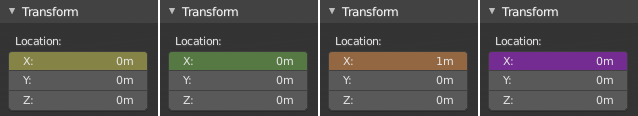
\includegraphics[width=0.7\textwidth]{blender_docs_images/animation_introduction_state-colors.png}
\end{center}

\begin{longtable}{cl}
    \toprule
    \textbf{Color} & \textbf{Meaning}                 \\
    \midrule
    \endhead
    \bottomrule
    \endfoot

    Gray           & Not animated                     \\
    Yellow         & Changed from the current frame   \\
    Green          & Keyframed on a different frame   \\
    Orange         & Changed from the keyframed value \\
    Purple         & Controlled by a \textit{Driver}  \\
\end{longtable}

\subsubsection{Rigging}

Rigging = adding controls handles to animate an object. Blender offers the following feature to rig a model
\begin{longtable}{p{0.2\textwidth}p{0.7\textwidth}}
    \toprule
    \textbf{Rigging Method}   & \textbf{Brief}                                                                                                                                                                                                                                                                                                         \\
    \midrule
    \endhead
    \bottomrule
    \endfoot

    \textbf{Armatures}        & A Hierarchy of Joints associated with a mesh. Each joint has a *weight* [0.0, 1.0] for each vertex of the aforementioned mesh (can be painted). Transforming a joint will influence all vertices whose weight for that particular joint is greater than 0. This technique is called *Skeletal Animation* (more later). \\
    \textbf{Constraints}      & Control the kind of motion the rig is allowed to perform. They are found under \textit{Properties Editor}, tab "Constraints" (more later).                                                                                                                                                                             \\
    \textbf{Object Modifiers} & Mesh deformation through modifiers. We are interested in \href{https://docs.blender.org/manual/en/4.3/modeling/modifiers/deform/index.html}{Deformations} and \href{https://docs.blender.org/manual/en/4.3/modeling/modifiers/physics/index.html}{Physics} (more later).                                               \\
    \textbf{Shape Keys}       & Commonly called textit{blendshape}, meaning having different copies of a mesh (same topology, same UV, same *everything*). Example: different facial expressions that blend over time with \textit{Keyframing} (more later).                                                                                           \\
    \textbf{Drivers}          & Mechanisms to control multiple properties at once and make some properties automatically update when others change (more later).                                                                                                                                                                                       \\
\end{longtable}

\subsection{Keyframes}

\subsubsection{Relevant Shortcuts}
\textbf{With a property/object Selected:}
\begin{longtable}{ll}
    \toprule
    \textbf{Shortcut}  & \textbf{Effect}                                \\
    \midrule
    \endhead
    \bottomrule
    \endfoot

    \textbf{I}         & Insert Keyframe (brings up keyframe menu)      \\
    \textbf{Alt + I}   & Delete Keyframe                                \\
    \textbf{Shift + I} & Insert Keyframe for all properties             \\
    \textbf{Ctrl + I}  & Add keyframe to active keying set              \\
    \textbf{Alt + S}   & Reset Scale (useful when animating transforms) \\
    \textbf{Alt + R}   & Reset Rotation                                 \\
    \textbf{Alt + G}   & Reset Location                                 \\
\end{longtable}
\textbf{Inside \textit{Graph Editor} or \textit{Dope Sheet Editor}}
\begin{longtable}{ll}
    \toprule
    \textbf{Shortcut}             & \textbf{Effect}                                             \\
    \midrule
    \endhead
    \bottomrule
    \endfoot

    \textbf{G}                    & Move keyframe(s)                                            \\
    \textbf{S}                    & Scale keyframe(s)                                           \\
    \textbf{R}                    & Rotate keyframe handle (in Graph Editor)                    \\
    \textbf{Shift + D}            & Duplicate keyframe(s)                                       \\
    \textbf{X} or \textbf{Delete} & Delete keyframe(s)                                          \\
    \textbf{E}                    & Extrapolate (Graph Editor)                                  \\
    \textbf{T}                    & Set Keyframe Interpolation (Linear, Bezier, Constant, etc.) \\
    \textbf{V}                    & Set Keyframe Handle Type (Vector, Aligned, etc.)            \\
    \textbf{Ctrl + C}             & Copy Keyframe                                               \\
    \textbf{Ctrl + V}             & Paste Keyframe                                              \\
\end{longtable}

\textbf{Playback Shortcuts}
\begin{longtable}{ll}
    \toprule
    \textbf{Shortcut}                   & \textbf{Effect}                                               \\
    \midrule
    \endhead
    \bottomrule
    \endfoot

    \textbf{Spacebar}                   & Play/Pause animation                                          \\
    \textbf{Shift + Left Arrow}         & Jump to \textbf{start frame}                                  \\
    \textbf{Shift + Right Arrow}        & Jump to \textbf{end frame}                                    \\
    \textbf{Left Arrow}                 & Move \textbf{one frame backward}                              \\
    \textbf{Right Arrow}                & Move \textbf{one frame forward}                               \\
    \textbf{Up Arrow}                   & Move to \textbf{next keyframe}                                \\
    \textbf{Down Arrow}                 & Move to \textbf{previous keyframe}                            \\
    \textbf{Shift + Ctrl + Spacebar}    & Play animation in \textbf{reverse}                            \\
    \textbf{Home}                       & Zoom to fit all keyframes in \textbf{Graph Editor/Dope Sheet} \\
    \textbf{Ctrl + Middle Mouse Scroll} & Zoom in/out in Timeline/Graph Editor                          \\
\end{longtable}
When you set a keyframe on a simple static mesh, like a cube. \\ (in the Viewport, object mode, Ctrl + A -> Mesh -> Cube). If
\begin{itemize}[topsep=0pt, noitemsep]
    \item You press \textbf{I}, then all the transform properties are saved in the current frame as a keyframe (see in \textit{Dope Sheet Editor})
    \item If you want only a part of the default properties to be saved, then you can set them manually by clicking the \textit{Animate Property} handle to
          the right of the property in the \textit{Properties Editor}
          \begin{center}
              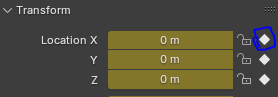
\includegraphics[width=0.4\textwidth]{blender_docs_images/my_properties_animate_handle.png}
          \end{center}
\end{itemize}

\subsubsection{Introduction}
A \textit{Keyframe} is a marker of time which stores the value of the selected property.\\
The purpose of a keyframe is to save the value of a property in a given instance of "time" (on a rendered frame. Physical elapsed time depends on the FPS of the animation).\par

An overview of all the existing keyframe in your animation can be seen in the \textit{Playback Editor}. To get the full information about existing keyframes (ie. to which
object they refer to and which property they alter/set, use the \textit{Dope Sheet Editor}).
\begin{center}
    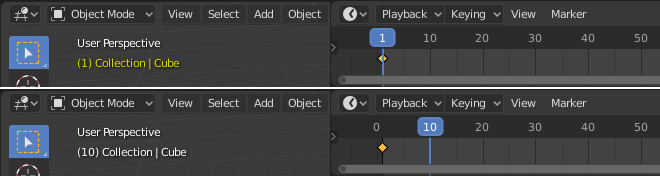
\includegraphics[width=0.7\textwidth]{blender_docs_images/animation_keyframes_introduction_visualization.png}
\end{center}
\begin{mdframed}[linewidth=2pt, linecolor=gray, roundcorner=1pt, innermargin=2pt, outermargin=2pt]
    \textbf{\Large Quick Experiment: Keyframe Visualization} \\[6pt]
    \textbf{File:} \texttt{01\_Keyframes\_Intro-Moving\_Cube.blend} \\[6pt]

    \begin{enumerate}[topsep=0pt, noitemsep]
        \item Create an empty Blender scene with a cube and check FPS \\
              (\textit{Properties Editor} $\rightarrow$ Output $\rightarrow$ Frame Rate).
        \item Select its position from the \textit{Properties Editor} and set a keyframe (\textbf{I} to keyframe the transform).
        \item Move to another keyframe inside \textit{Dope Sheet Editor} or \textit{Playback Editor}.
        \item Freely transform your cube and then set a keyframe. \\
              \textbf{Note:} It's imperative that you first move to another place in the timeline and then manipulate your object, otherwise it won't work!
        \item Go back to the start of the timeline (\textbf{Shift + Left Arrow}) and play the animation (\textbf{Spacebar}).
    \end{enumerate}

    \textit{Keep this example for the next section on Interpolation.}
\end{mdframed}

\subsubsection{Interpolation}
When you set two keyframes on the same property, its value changes over the span of frames inbetween the two keyframes with \textit{Interpolated Values}, ie values computed using
a matematical formula. In particular, such formula is defined by an \href{https://docs.blender.org/manual/en/4.3/editors/graph_editor/fcurves/introduction.html}{\textit{F-Curve}},
manipulated in the \textit{Graph Editor}.
\begin{center}
    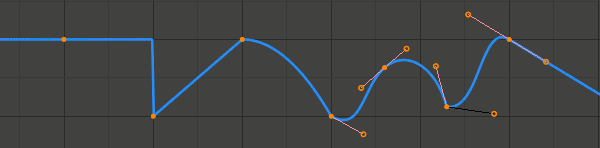
\includegraphics[width=0.7\textwidth]{blender_docs_images/animation_keyframes_introduction_curves.png}
\end{center}

There is 1 curve for each animated property in the \textit{Dope Sheet Editor}. The main setting is the \textit{Interpolation} Type, which appears in the \textit{Graph Editor} inside the
\textit{F-Curve} Tab. \textbf{Interpolation Modes:}\footnote{All the settings inside the \textit{F-Curve} Tab affect the keyframes selected}
\begin{itemize}[topsep=0pt, noitemsep]
    \item Bezier Curve
    \item Linear
    \item Constant
\end{itemize}
\begin{center}
    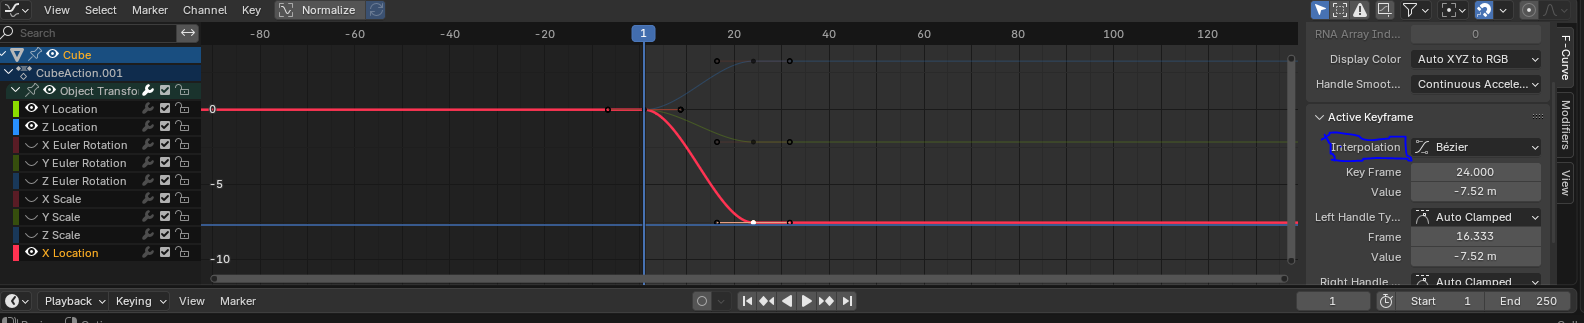
\includegraphics[width=0.9\textwidth]{blender_docs_images/my_graph_editor_interpolation_mode.png}
\end{center}
While what happens during the transition between a keyframe and the next one is defined by the \textit{Interpolation} Mode, What happens outside the "Keyframed Range"
(before the first keyframe and after the last keyframe) is defined by the \textit{Extrapolation Mode}.\par
\textit{Extrapolation Mode} is found under \mbox{"\textit{Graph Editor}/Channel/Extrapolation Mode"} or with shortcut \textbf{Shift + E} (\textit{Graph Editor} Selected)
The following are the available \textbf{Extrapolation Modes:}\footnote{Extrapolation Mode affects all \textit{F-Curves} selected}
\begin{itemize}[topsep=0pt, noitemsep]
    \item Constant: Continue in a straight horizontal line
    \item Linear: Continue in a straight line keeping the slope
    \item Make Cyclic: Repeat the curve
    \item Clear Cyclic: Removes Cycles Modifier
\end{itemize}

The settings to manipulate Curve Handles (placed on the F-Curve on the keyframe positions) depend on the Interpolation Type. A common setting among them all is the
\textit{Auto Handle Smoothing}, which can be either \textit{None} or \textit{Continuous Acceleration}.\par
When not \textit{None}, edits to a handle are propagated in the near handles (similiar to proportional editing) to keep the F-Curve as smooth as possible.
\begin{mdframed}[linewidth=2pt, linecolor=gray, roundcorner=1pt, innermargin=2pt, outermargin=2pt]
    \textbf{\Large Quick Experiment: Interpolation and Extrapolation: "Cyclic Overshoot"} \\[6pt]
    \textbf{File:} \texttt{02\_Keyframes\_Interpolation-Moving\_Cube\_Custom\_Interpolation.blend} \\[6pt]

    \begin{enumerate}[topsep=0pt, noitemsep]
        \item Open the cube example you produced from the previous experiment
        \item Open the \textit{Graph Editor} and select a "Location" Curve (the one with the bigger displacement in the Vertical axis)
        \item Play around with the 2 Handles freely. Example: Use the last one as "Bezier" Interpolation and create an "overshoot"
        \item Change the \textit{Extrapolation mode} to Linear and then to Make Cyclic
        \item Check in the "\textit{Graph Editor}/Modifiers" (Tab) that The Cycles Modifier has been added to the \textit{F-Curve}
        \item Go back to the start of the timeline (\textbf{Shift+Left Arrow}) and play the animation (\textbf{Spacebar})
    \end{enumerate}

    \textit{Keep this example for the next section on Interpolation.}
\end{mdframed}

\subsubsection{Keyframe Types}

\section{Animation: Used Editors}
\subsection{Properties Editor}

\subsection{Playback Editor}

\subsection{Dope Sheet Editor}

\subsection{Graph Editor}

\section{Animation Scenario: Camera Rig}

\end{document}
